\section{Evaluación}

\begin{frame}{Pruebas preliminares}

\begin{figure}
    \begin{subfigure}[b]{.5\linewidth}
        \centering
        \includegraphics[height=3cm]{../resultados/imagenes/interfaz_tiempo_actividades.png}
        \caption{Tiempo por tipo de actividad}
    \end{subfigure}\hfill
    \pause
    \begin{subtable}[b]{.5\linewidth}
        \tiny
        \centering
        \begin{tabular}{lr}
        \toprule
        Métrica & Disconformidad \\
        \midrule
        Calidad Gráfica         & {\color{green!90!black} 0.17} \\
        Interacción Entorno     & {\color{red!90}   0.50} \\
        Interacción Objetos     & {\color{red!90}   0.49} \\
        Características Entorno & {\color{green!90!black} 0.33} \\
        Usabililidad Interfaz   & {\color{red!90}   0.51} \\
        Integración Hardware    & {\color{green!90!black} 0.27} \\
        \bottomrule
        \end{tabular}
        \caption{Disconformidad por métrica}
    \end{subtable}
\end{figure}

\end{frame}
\begin{frame}{Encuesta determinar muestra}

\begin{figure}
    \begin{subfigure}[b]{.3\linewidth}
        \centering
        \includegraphics[height=2cm]{../resultados/imagenes/ubicacion_acceso_internet.png}
        \caption{Acceso a internet}
    \end{subfigure}\hfill
    \pause{}
    \begin{subfigure}[b]{.3\linewidth}
        \centering
        \includegraphics[height=2cm]{../resultados/imagenes/ubicacion_sistemas_operativos.png}
        \caption{Sistema operativo}
    \end{subfigure}\\
    \pause{}
    \begin{subfigure}[b]{.5\linewidth}
        \centering
        \includegraphics[height=2cm]{../resultados/imagenes/ubicacion_requisitos_minimos.png}
        \caption{Cumplimiento de requisitos}
    \end{subfigure}
\end{figure}

\end{frame}

\begin{frame}[t,fragile]
\frametitle{Encuesta para evaluar conocimiento (I)}
\centering

% Datos
\begin{filecontents}{objetiva.dat}
n	total        muestra	    control
1	0.2020159639 0.3636363636	0.1818181818
2	0.6027491017 0.6363636364	0.6
3	0.1332966457 0.09090909091	0.1363636364
4	0.2580191298 0.2727272727	0.2545454545
5	0.5869865976 0.8181818182	0.5636363636
6	0.1640933841 0	            0.1834862385
7	0.5256475617 0.6363636364	0.5137614679
8	0.2947317706 0.4545454545	0.2752293578
9	0.3081905611 0.1818181818	0.3211009174
10	0.4498120076 0.3636363636	0.4587155963
\end{filecontents}
\pgfplotstableread{objetiva.dat}{\Objetiva}

\begin{tikzpicture}
\begin{axis}[
    title={},
    xlabel={Pregunta},
    ylabel={Puntos},
    xmin=1, xmax=10,
    ymin=0, ymax=1,
    xtick={0,1,2,3,4,5,6,7,8,9,10},
    ytick={0,.25,.50,.75,1},
    legend pos=outer north east,
    ymajorgrids=true,
    xmajorgrids=true,
    grid style=dashed,
]
 
\only<1->{\addplot[color=blue,] table [x = {n}, y = {muestra}] {\Objetiva};
\addlegendentry{Muestra}}
\only<2->{\addplot[color=red,] table [x = {n}, y = {control}] {\Objetiva};
\addlegendentry{Control}}
\only<3->{\addplot[color=black,dashed] table [x = {n}, y = {total}] {\Objetiva};
\addlegendentry{Total}}
 
\end{axis}
\end{tikzpicture}

\end{frame}
\begin{frame}
\frametitle{Encuesta para evaluar conocimiento (II)}

\begin{table}
\begin{tabular}{lr}
\toprule
Promedio usuarios & \textbf{3.82} \\
\onslide+<2->{Promedio control  & \textbf{3.47} \\\midrule}
\onslide+<3->{Promedio total    & \textbf{3.49}}
\\\bottomrule
\end{tabular}
\caption{Puntaje promedio por grupo}
\end{table}
\note{Estos datos no son estadísticamente válidos}
\note{El Incrmeento es del $10\%$}

\end{frame}
\begin{frame}{Encuesta para evaluar la solución (I)}

\begin{figure}
    \scriptsize
    \centering
    \begin{subtable}[b]{.5\linewidth}
        \tiny
        \begin{tabular}{lc}
        \toprule
        Factores                 & Promedio encuesta \\
        \midrule
        Motivación               & De acuerdo \\
        Facilidad de exploración & De acuerdo \\
        Sensación de Inmersión   & De acuerdo \\
        Pedagogía                & De acuerdo \\
        Representación           & Parcialmente de acuerdo \\
        Retroalimentación        & Parcialmente de acuerdo \\
        Utilidad                 & De acuerdo \\
        \bottomrule
        \end{tabular}
        \caption{Aceptación por aspecto de la solución}
    \end{subtable}\hfill
    \pause
    \begin{subfigure}[b]{.5\linewidth}
        \tiny
        \begin{tikzpicture}[label distance=.15cm]
        \tkzKiviatDiagram[scale=.4,%
                            lattice=9,
                            %step=10,
                            ]
                        {Motivación,
                         Exploración,
                         Inmersión,
                         Pedagogía,
                         Representación,
                         Retroalimentación,
                         Utilidad}
        \tkzKiviatLine[thick,
                        color=blue!25!white,
                        mark=ball,
                        ball color=blue,
                        mark size=5pt,
                        opacity=.2, 
                        fill=blue!20](6.7,6.8,6.3,6.7,5.3,6.0,6.9)
        \tkzKiviatGrad[prefix={$0,$},unity=1](1) 
        \end{tikzpicture}
        \caption{Valores estandarizados}
    \end{subfigure}
\end{figure}

\end{frame}
\begin{frame}{Encuesta para evaluar la solución (II)}


\begin{table}
\scriptsize
\centering
\begin{tabular}{lcr}
\toprule
& \multicolumn{2}{c}{Promedio} \\
%\cmidrule(c){2-3} 
\cmidrule(lr){2-3}
Hipótesis                        & Encuesta                & Estandarizado \\
\midrule
Comandos de voz con interfaz     & De acuerdo              & $0,55$ \\
Extracción uniforme de elementos & Parcialmente de acuerdo & $0,65$ \\
Acciones de bioseguridad         & De acuerdo              & $0,58$ \\
Representación iconográfica      & Parcialmente de acuerdo & $0,53$ \\
Factores motivadores             & De acuerdo              & $0,65$ \\
Falta de pistas                  & De acuerdo              & $0,61$ \\
\bottomrule
\end{tabular}
\caption{Aceptación por hipótesis}
\end{table}

\end{frame}

\begin{frame}{Registro de actividades (I)}

\begin{table}
\centering
\small
\begin{tabular}{lr}
\toprule
Partidas                         & 99 \\
Primera partida                  & 4 de Noviembre de 2014 \\
Última partida                   & 23 de Noviembre de 2014 \\
\midrule
\onslide+<2->{Tiempo total                     & 11.134 \\
Promedio de tiempo por partida   & 112}
\\\midrule
\onslide+<3->{Acciones                         & 2.944 \\
Promedio de acciones por partida & 30}
\\\midrule
\onslide+<4->{Usuarios                         & \textcolor{red}{8} \\
Promedio de partidas por usuario & 12}
\\\bottomrule
\end{tabular}
\caption{Utilización de la solución}
\end{table}

\end{frame}
\begin{frame}[t,fragile]
\frametitle{Registro de actividades (II)}

%Datos
\begin{filecontents}{registrohemocultivo.dat}
n   p   s
 1  11  14.3
 2  9   10.6
 4  3   3.3 
 5  3   6.8 
 6  3   5.8 
 7  4   4   
 9  16  0
10  3   7.2 
\end{filecontents}

\pgfplotstableread{registrohemocultivo.dat}{\RegHemocultivo}

\begin{figure}
\centering
\begin{tikzpicture}[scale=.85]
   \begin{axis}[ybar,%
      legend pos=outer north east,
      symbolic x coords={1,2,4,5,6,7,9,10},
      ymin=0,ymax=18,
      xtick=data,
      ytick={0,3,6,9,12,15,18},
      ylabel= Puntaje,
      xlabel= Alumno,
      bar width=6pt,
        ]   
\addplot[color=blue,ybar,fill=blue!75,area legend] table [x = {n}, y = {p}] {\RegHemocultivo};
\addlegendentry{Primer}
\addplot[color=red,ybar,fill=red!75,area legend] table [x = {n}, y = {s}] {\RegHemocultivo};
\addlegendentry[align=left]{Promedio \\ siguientes}
\end{axis}
\end{tikzpicture}
\caption{Puntaje \emph{Extracción de sangre}}
\end{figure}

\end{frame}
\begin{frame}[t,fragile]
\frametitle{Registro de actividades (III)}

%Datos
\begin{filecontents}{registroglasgow.dat}
n    p    s
1    1    1.5 
2    2    2.3 
4    1    1.5 
6    2    2 
7    0    1 
\end{filecontents}
\pgfplotstableread{registroglasgow.dat}{\RegGlasgow}

\begin{figure}
\centering
\begin{tikzpicture}[scale=.85]
   \begin{axis}[ybar,%
      legend pos=outer north east,
      symbolic x coords={1,2,4,6,7},
      ymin=0,ymax=4,
      xtick=data,
      ytick={0,1,2,3,4},
      ylabel= Puntaje,
      xlabel= Alumno,
        ]   
\addplot[color=blue,ybar,fill=blue!75,area legend] table [x = {n}, y = {p}] {\RegGlasgow};
\addlegendentry{Primer}
\addplot[color=red,ybar,fill=red!75,area legend] table [x = {n}, y = {s}] {\RegGlasgow};
\addlegendentry[align=left]{Promedio \\ siguientes}
\end{axis}
\end{tikzpicture}
\caption{Puntaje \emph{Evaluación Glasgow}}
\end{figure}

\end{frame}
\begin{frame}{Correlación}


\begin{table}
\scriptsize
\centering
\begin{tabular}{lrc}
\toprule
Factores                                                    & Valor         & Interpretación \\
\midrule
\onslide+<1->{Tiempo de uso y puntaje máximo extracción     & \textbf{0.62} & Positiva Fuerte}\\
\onslide+<2->{Tiempo de uso y puntaje máximo glasgow        & \textbf{0.78} & Positiva Muy Fuerte}\\
\onslide+<3->{Puntaje máximo extracción y encuesta objetiva & \textbf{0.44} & Positiva Fuerte}\\\bottomrule
\end{tabular}
\end{table}

\end{frame}
